\subsection{Colorimetry and Colour Measurement}

\textit{The current recommended source for colorimetry is \gls{CIE} document `\gls{CIE} 015:2018'\citep{cie_cie_2018}\footnote{Though as \citet{fairchild_cie_2019} notes, this document is `expensive and somewhat difficult to find', and as such I have been using a draft of the now superseded `\gls{CIE} 15.3:2004'\citep{cie_cie_2004-2} as my personal guide.}. Whlist this is the authoritative reference, my personal opinion is that an understanding of colorimetry of \gls{CIE} colorimetry is best gained from an understanding of it's history, and for this I recommend Janos Schanda's book `Colorimetry: Understanding the \gls{CIE} System'\citep{schanda_colorimetry_2007}.}

\bigskip

Colorimetry is the study of the quantitative specification of colour. As a subjective, internal and anthropocentric concept, in order to measure anything meaningful and comparable, we use a standard observer, or more precisely, one of a number of defined standard observers \cite{cie_bs_2011}.

The classic standard observer was defined by the \gls{CIE} in 1931, following experiments by Wright and Guild \cite{wright_re-determination_1929, guild_colorimetric_1931}. Despite several more recently published standard observers, the 1931 observer is still much used, and I shall use it in the following example of how a basic colorimetric computation is performed.

An illuminant is defined by its \gls{SPD}, a surface as it's \gls{SRF}, and a the sensitivity of a sensor (such as a photosensitive cell in the retina, or a pixel in a camera) by its \gls{CMF} (or in the case that biologically based measurements are used - the \gls{SSF}).

\begin{figure}[htbp]
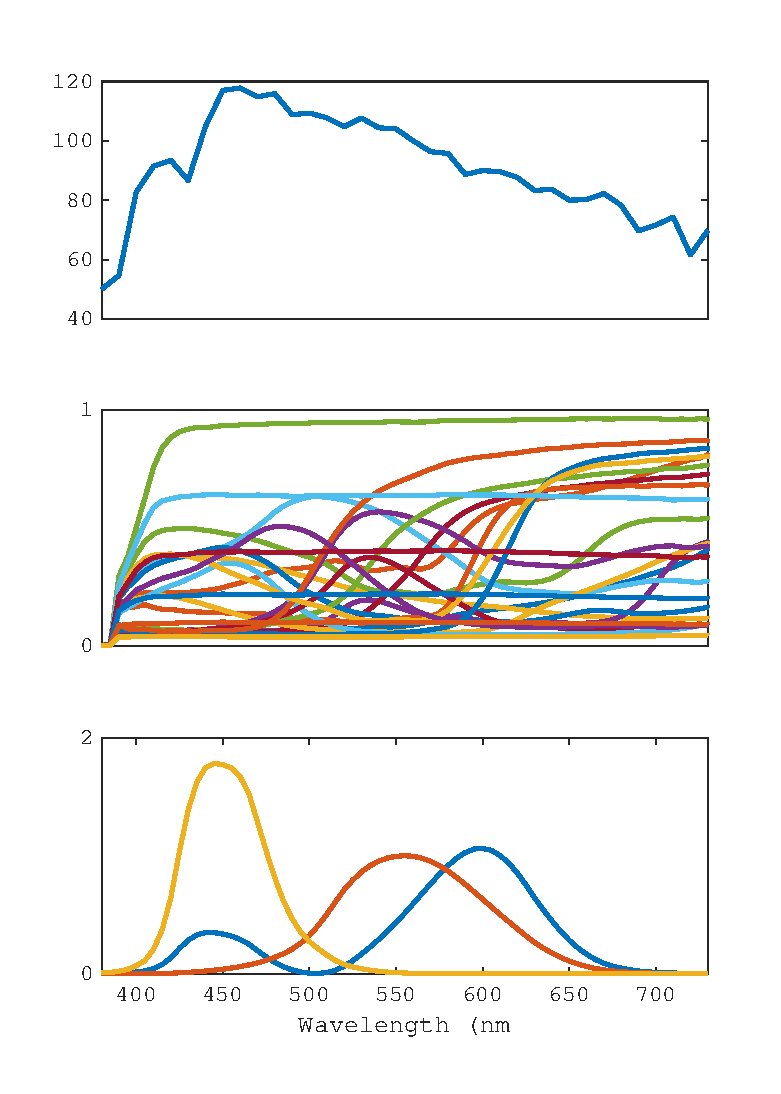
\includegraphics[max width=\textwidth]{figs/LitRev/SPDetc.pdf}
\caption{An \gls{SPD} (D65), a set of \glspl{SRF} (from a Macbeth Colour Checker) and three \glspl{CMF} (\gls{CIE} 1931).}
\label{fig:specFun}
\end{figure}
% % How is D65 normalised here?

The light reaching the eye for a given reflecting surface under a given illuminant (termed the `colour signal') can be computed by multiplying the \gls{SPD} by the \gls{SRF} at each sampled interval.

\begin{equation}
\phi(\lambda)=R(\lambda) \cdot S(\lambda)
\end{equation}

where $R(\lambda)$ is the \gls{SRF}, $R(\lambda)$ is the \gls{SPD} and $\phi(\lambda)$ is the resulting colour signal. From this a set of values termed `tristimulus values' may be computed. Tristimulus values are computed by multiplying the colour signal by the \glspl{CMF} or \glspl{SSF}, and following the principle of univariance (that each cone type cannot alone distinguish between different wavelengths) the tristimulus values can, to some extent, be thought of as containing the entirety of the chromatic information about a surface (excluding high level colour appearance phenomena predicted by \Glspl{CAM}, and properties such as gloss).

\begin{subequations}
\begin{align}
X=k \sum_{\lambda} \phi(\lambda) \overline{x}(\lambda) \Delta \lambda \\ 
Y=k \sum_{\lambda} \phi(\lambda) \overline{y}(\lambda) \Delta \lambda \\ 
Z=k \sum_{\lambda} \phi(\lambda) \overline{z}(\lambda) \Delta \lambda
\end{align}
\label{eq:XYZ}
\end{subequations}

where $\overline{x}(\lambda)$ (said `x bar'), $\overline{y}(\lambda)$ and $\overline{z}(\lambda)$ are the \glspl{CMF} of the 1931 observer (or are replaced by the \Glspl{CMF}/\Glspl{SSF} or the chosen observer), $\phi(\lambda)$ is as defined above, $k$ is a normalising factor, and it is recommended that $\Delta\lambda$ be 1nm. It is traditional to set $k$ such that $Y=100$, though in the case of relative colorimetry (most cases) is often ignored since the following equation renders it superfluous.

From the tristimulus values chromaticity co-ordinates ($x$ and $y$) can be computed. These can then be plotted on a 1931 chromaticity diagram, shown as Figure \ref{fig:1931}.

\begin{subequations}
\begin{align}
x=\frac{X}{X+Y+Z} \\
y=\frac{Y}{X+Y+Z} 
\end{align}
\label{eq:1931chrom}
\end{subequations}

% Here's a \gls{MATLAB} example, using \gls{PTB} for data:

% \begin{lstlisting}[language=MATLAB]
% load spd_D65 % SPD: CIE D-series illuminant D65
% load sur_macbeth % SRF: macbeth colour checker
% load T_xyz1931 % CMF: CIE 1931

% colourSignals = sur_macbeth.*spd_D65;
% XYZ = T_xyz1931*colourSignals;
% xy = [XYZ(1,:)./sum(XYZ);XYZ(2,:)./sum(XYZ)];
% \end{lstlisting}

% Plotting: 

% \begin{lstlisting}[language=MATLAB]
% spectralLocus = [T_xyz1931(1,:)./sum(T_xyz1931);T_xyz1931(2,:)./sum(T_xyz1931)];
% sRGBSpectralLocus = XYZToSRGBPrimary(T_xyz1931);

% figure, hold on, 
% scatter(spectralLocus(1,1:70),spectralLocus(2,1:70),[],sRGBSpectralLocus(:,1:70)','filled')
% scatter(xy(1,:),xy(2,:),'k')
% axis equal, axis([0 1 0 1])
% xticks([0 1]), yticks([0 1])
% xlabel('x'), ylabel('y')
% \end{lstlisting}

\begin{figure}[htbp]
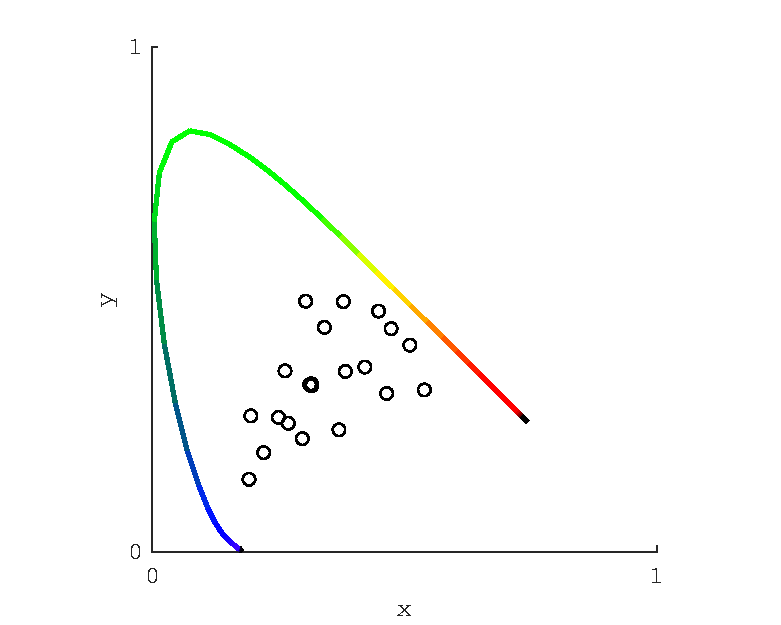
\includegraphics[max width=\textwidth]{figs/LitRev/ColorimetryDemo1.pdf}
\caption{The \gls{CIE} 1931 chromaticity diagram, showing the chromaticity of the macbeth colour checker patches under D65. Note that for all of the plots in this section, the colours used for the spectral loci are only very rough approximations.}
\label{fig:1931}
\end{figure}

\subsubsection{Specific Colour Spaces}

Over time various other colour spaces have been proposed and formally accepted by the \gls{CIE}, each aiming to improve upon a prior space in one or more ways. One of the most frequently sought characteristics for a colour space is perceptual uniformity, whereby a set distance in one part of the space is comparable in terms of apparent colour difference to that same distance in another part of the space.

One such chromaticity space which shall be used extensively in this thesis is the \gls{CIE} 1976 UCS (uniform chromaticity scale) diagram, which is a relatively simple transformation of the 1931 chromaticity diagram. The conversion can be accomplished in a number of analogous fashions, one of which is shown below.

\begin{subequations}
\begin{align}
u' &= 4x / (-2x + 12y + 3) \\
v' &= 9y / (-2x + 12y + 3)
\end{align}
\end{subequations}

where $x$ and $y$ are the 1931 chromaticity co-ordinates as defined in Equation \ref{eq:1931chrom}. The data presented in Figure \ref{fig:1931} are re-plotted in this new space in Figure \ref{fig:UCS}.

\begin{figure}[htbp]
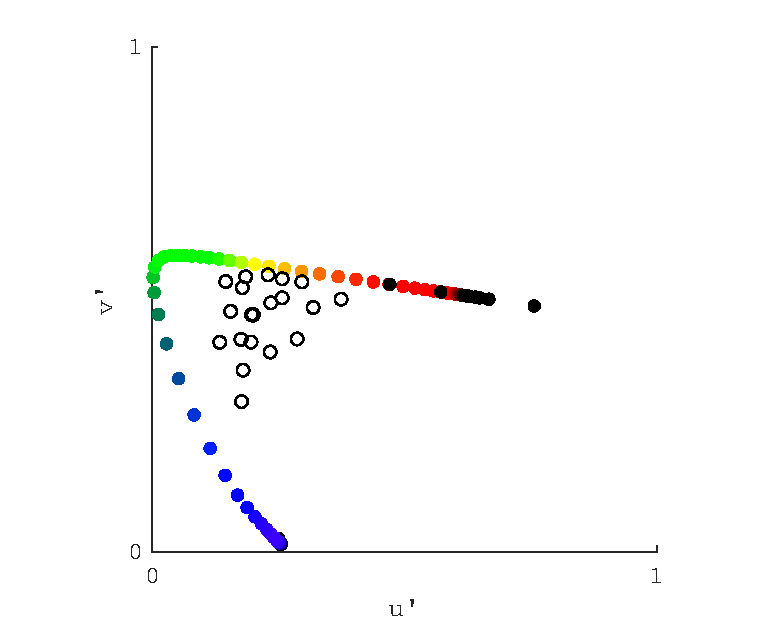
\includegraphics[max width=\textwidth]{figs/LitRev/ColorimetryDemo3.pdf}
\caption{\gls{CIE} 1976 UCS (uniform chromaticity scale) diagram, showing the chromaticity of the macbeth colour checker patches under D65 (as in Figure \ref{fig:1931}).}
\label{fig:UCS}
\end{figure}

A three-dimensional extension to the CIE 1976 UCS diagram is the \gls{CIE} 1976 L*u*v* colour space, often abbreviated to CIELUV, which aims to provide perceptual uniformity in a space that includes both chromaticity and lightness (relative to a white object under the same illumination). It is defined as follows:

\begin{subequations}
\begin{align}
L^{*} &= 116 f(Y/Y_{n})-16 \\
\textrm{where} f(Y/Y_{n}) &= (Y/Y_{n})^{1/3} &\textrm{ if } (Y/Y_{n}) > (24/116)^{3} \\
\textrm{where} f(Y/Y_{n}) &= (841/108)(Y/Y_{n})+16/116 &\textrm{ if } (Y/Y_{n}) \leq (24/116)^{3} \\
u^{*} &= 13L^{*}(u'-u'_{n}) \\ 
v^{*} &= 13L^{*}(v'-v'_{n})
\end{align}
\end{subequations}

where $Y_{n}$, $u'_{n}$ and $v'_{n}$ refer to the colour stimulus of a perfect reflector. The same data presented in Figures \ref{fig:1931} and \ref{fig:UCS} is presented in CIELUV in Figure \ref{fig:CIELUV} (though of course the three-dimensional quality of the data is somewhat lost).

\begin{figure}[htbp]
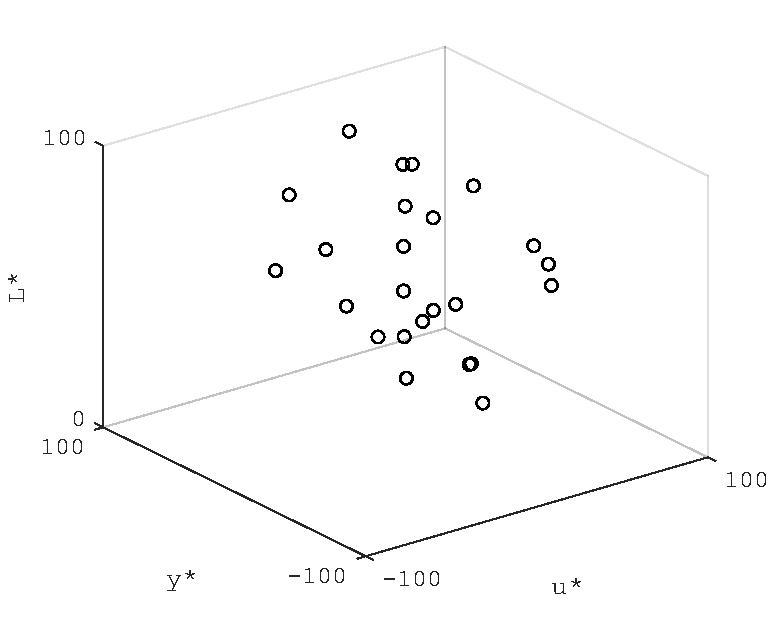
\includegraphics[max width=\textwidth]{figs/LitRev/ColorimetryDemo4.pdf}
\caption{A representation of CIELUV, showing the values for the macbeth colour checker patches under D65 (as in Figure \ref{fig:1931} and \ref{fig:UCS}). Note that if viewed from above, the distribution of points would appear similar to as in Figure \ref{fig:UCS}. If all of the points were of uniform L*, then the distribution would be identical, only with different scaling.}
\label{fig:CIELUV}
\end{figure}

The final colour space presented here is the \acrfull{MB} colour space. This space does not aspire to be perceptually uniform\footnote{This can be clearly noted by comparing Figure \ref{fig:lrMB} with previous figures. Where this set of chromaticities previously spanned the spaces fairly broadly, here all the chromaticities inhabit only a small portion of the chromaticity space.}. Instead, it aspires to provide a colour space which has a physiological underpinning. As such, the observer used consists of nominal \glspl{SSF} (rather than \glspl{CMF}), and the conversion from tristimulus values to chromaticity space attempts to mirror the way in which this actually occurs physiologically.

It was originally proposed by \citet{macleod_chromaticity_1979}, but was recently revised and endorsed by the \gls{CIE}, in documents `CIE 170-1:2006'\citep{cie_cie_2006} and `CIE 170-2:2015'\citep{cie_cie_2015}\footnote{I understand that the final publication in the series (`CIE 170-3:XXXX') is in preparation.}. The revisions included the definition of a new observer, based on the work of \citet{stockman_spectral_1999} and \citet{stockman_spectral_2000}, and the introduction of a set of new normalising terms, such that it is now calculated as follows.

\begin{subequations}
\begin{align}
L_{\text{MB}}&=k_{l} \sum_{\lambda} \phi(\lambda) \overline{l}(\lambda) \Delta \lambda \\ 
M_{\text{MB}}&=k_{m} \sum_{\lambda} \phi(\lambda) \overline{m}(\lambda) \Delta \lambda \\ 
S_{\text{MB}}&=k_{s} \sum_{\lambda} \phi(\lambda) \overline{s}(\lambda) \Delta \lambda
\end{align}
\label{eq:MBTristim}
\end{subequations}

where $k_{l}$ = 0.68990272, $k_{m}$ = 0.34832189, $k_{s}$ = 0.03715971. This set differs minimally but purposefully from Equation \ref{eq:XYZ}; in the choice of observer ($\overline{lms}$), and in the use of different scaling factors for each tristimulus value. \gls{MB} chromaticity values are then calculated as follows:

\begin{subequations}
\begin{align}
l_{\text{MB}}&= \frac{L_{\text{MB}}}{L_{\text{MB}}+M_{\text{MB}}} \\ 
s_{\text{MB}}&= \frac{S_{\text{MB}}}{L_{\text{MB}}+M_{\text{MB}}} 
\end{align}
\label{eq:MB}
\end{subequations}

Whereas the relationship between the axes of previous colour spaces was important, here the axes are nominally independent (representing different post-receptoral mechanisms) and so the scaling between the axes is arbitrary. The same data as presented previously is presented again in Figure \ref{fig:lrMB} in a \gls{MB} chromaticity space.

\begin{figure}[htbp]
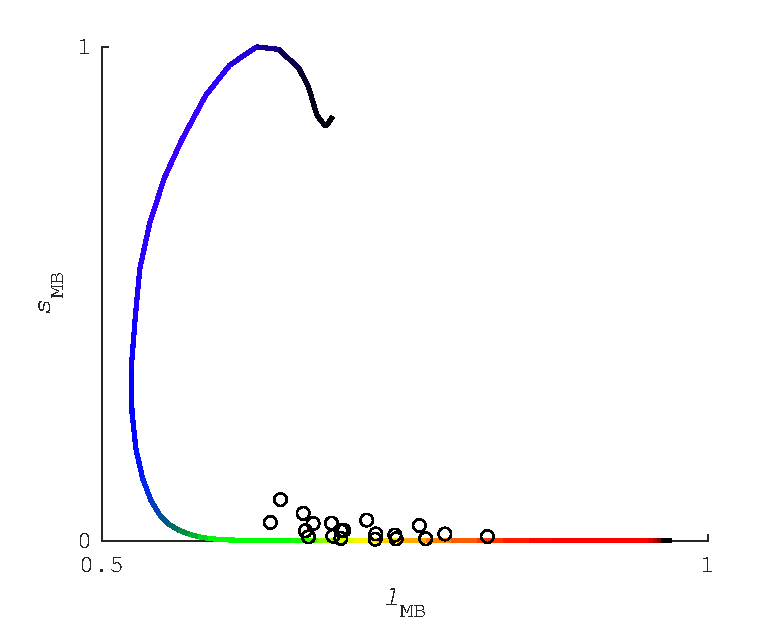
\includegraphics[max width=\textwidth]{figs/LitRev/ColorimetryDemo5.pdf}
\caption{A \gls{MB} chromaticity diagram (as per \gls{CIE} 170-2:2015\citep{cie_cie_2015}) showing the values for the macbeth colour checker patches under D65, as in previous figures.}
\label{fig:lrMB}
\end{figure}

\clearpage